\documentclass[man,hidelinks,floatsintext]{apa7}
\raggedbottom
\usepackage{graphicx,color,soul,setspace}
\graphicspath{{./img/}}
\usepackage[autostyle,english=american]{csquotes}
\usepackage[american]{babel}
\usepackage[style=apa,backend=biber]{biblatex}
\bibliography{cites}
\title{Exploring Microarchitectures with LLAMA-16}
\shorttitle{LLAMA-16 MICROARCHITECTURE}
\author{Jaydin Andrews}
\authorsaffiliations{Department of Computer Science\\University of North Carolina at Asheville\\jandrew3@unca.edu}
\authornote{Thank you to my peers in Dr. Sanft's Systems II class. Your willingness to explore this project and provide feedback was invaluable. Thank you Dr. Sanft for giving me the opportunity to present this project in an educational setting.}
\abstract{Due to the complexity of assembly languages that have been continuously expanded on for over 75 years, students can easily become overwhelmed when attempting to learn these languages. They do not think that programming in assembly is much more akin to solving a sliding block puzzle than manipulating data with magnets and electricity. Puzzles are supposed to be fun yet stimulating; they should be easy to learn but offer limitless possibilities. LLAMA-16 is designed to be the teaching puzzle of assembly programming. With a stripped down RISC architecture, this virtual computer can be programmed to do nearly anything. Offering only sixteen instructions, LLAMA-16 scales back the intensity of the monolithic x86\_64 instruction set with its well over nine-hundred instructions. By reducing the complexity of standard assembly used in real world applications while still maintaining the same programming conventions and styles LLAMA-16 offers a unique toolset to help all students of computer science explore microarchitecture design in a digestible manner. Its entirely virtual emulator allows writing, running, and exploring assembly programs to be as easy as writing a text document. By lowering the barrier of entry to low level systems programming, it can only widen the net of lifelong students to help each other learn the fundamentals of computer science.}
\begin{document}
\maketitle
\section{Introduction}
LLAMA-16 is a 16-bit Instruction Set Architecture that can be used as an educational tool to introduce students to low level assembly programming. Designed to be digestible yet practical, LLAMA-16 features a manageable RISC instruction set rich in utility. The software implementations of this ISA feature a two-pass assembler and a machine emulator. Both tools have built in debugging options designed to provide an in-depth look into the machine's architecture. Users can explore parsing and assembling theory with the built-in options for verbose line-by-line parsing information. Students can view, line by line, their custom programs decoded and executed by the machine emulator. They can dive head first into machine architectures or they can simply explore assembly programming by writing their own programs.\par
LLAMA-16 features eight 16-bit registers, a fully addressable 16-bit memory space, a built-in stack, and memory-mapped I/O. Sixteen unique instructions offers the ability to fully interact with the machine without needing to reference pages of dense documentation. With a built-in stack and support for subroutines, students can explore the concepts of recursion and imperative programming. The entire project is open source and written in standard library Python making it accessible to nearly everyone. The instruction set is logically complete and Turing-equivalent; users are limited only by their own imagination.
\section{Background}
CISC and RISC minicomputers have been around for a long time. As a result, a number of similar projects to LLAMA-16 have been made. Detailed below are a few projects similar to LLAMA-16, but differ in either scope or implementation.
\paragraph{Little Man Computer}
The Little Man Computer is an instructional model of computer architecture. It was created by Dr. Stuart Madnick of the Massachusetts Institute of Technology in 1965 \parencite{lmc}. This model is a very simple computer based on the analogy of a little man shut in a closed mailroom: a wall of mailboxes act as memory, an inbox and an outbox are used to input and output data respectively. The analogy is a simple one but is an illustration of a von Neumann architecture, the basis for modern computation. A number of simulators have been made to demonstrate the LMC instruction set in use. The LMC is a great way to introduce the concepts of minicomputer design. The instruction set of the LMC is very limited; however this is by design. It was designed as a proof-of-concept educational project and not as a contender for minicomputer architectures.
\paragraph{Little Computer 3}
The Little Computer 3 was developed by Dr. Yale Patt of the University of Texas at Austin and Dr. Sanjay Patel of the University of Illinois at Urbana-Champaign. The LC-3 is a very simple instruction set architecture \parencite{lc3}. The specification states that the word size of registers is 16 bits, includes a 16-bit addressable memory space and has eight general-purpose registers. Of the sixteen bits that make up an instruction, four are used for opcodes. While it is used as a default non-x86 assembly language for educational purposes, the LC-3 uses relative offsets from the program counter to calculate memory addresses for instruction jumps. This reduces the complexity of having a program stack, however is not very scalable to large architectures in the x86 family. Some of this usability is enhanced in the next iteration of the project, the LC-3b. The stack is still not directly mutable, but loading and storing instructions uses register-based addressing instead of program counter relative addressing. This does not eliminate program counter relative addressing as it is still used for branching instructions. Program counter relative offsets require additional computation when jumping to new locations in memory and are encoded differently for every instruction. This means that a different set of procedural logic must be applied to the instruction to parse the offset and calculate the memory address before the execution of the instruction even begins.
\paragraph{MIPS}
Another set of machine architectures commonly seen in education is MIPS: Microprocessor without Interlocked Pipelined Stages. MIPS is a family of reduced instruction set computer instruction set architectures originally developed in 1981 by J. L. Hennessy for MIPS Computer Systems. These architecture designs were the first to pave the way for the later developed notion of RISC architectures. MIPS is generally taught in universities due to the multitude of simulators designed to show the inner workings of how the machine execution. While these visual representations are very helpful when learning, the language itself has outgrown its original design. MIPS architectures was never designed to be a learning tool, it was designed by MIPS Computer Systems for their brand new R2000 microprocessor released in 1985. Over the past forty years MIPS has been extensively expanded in its usability as well as its complexity. MIPS offers thirty-two 32-bit general purpose registers as well as another thirty-two 32-bit floating-point registers \parencite{mips}. In 1991, MIPS made the jump from 32-bit instructions to 64. This drastically complicated the instruction set making its use as a learning model stall until 32-bit versions of newer releases were introduced. One of the major pit-falls of learning with MIPS languages is the instruction form. Many other systems use the two opcode form where the second operand acts as both a source of data and the eventual destination of the resulting data. MIPS uses a three opcode format where the first two operands are for the source data, and the third is the destination of the result. This is one of the biggest hurdles students have to overcome when switching from MIPS to x86.
\paragraph{CFT Minicomputer}
The Copious Free Time home-brew minicomputer is a hobby project by GitHub user Alexios. It is an extensively designed homebuilt minicomputer entirely made from scratch. This project has been actively developed and maintained since 2011. This project also is based around a hardware implementation of the processor design \parencite{cft}. It has a 16-bit word size, much like LLAMA-16, simply for ease of use and understanding. Unlike the CFT, LLAMA-16 does not have a hardware implementation but rather an emulator for virtual execution of the machine's logic.
\paragraph{JDH-8}
In a similar category as the CFT project, the JDH-8 is also a from-scratch implementation of a minicomputer. This project also includes a hardware implementation of the machine. The difference between the CFT and JDH-8 is that jdah, the developer of the JDH-8, initially created an emulator before designing the hardware machine. The JDH-8 suite includes an assembler, emulator, hardware implementation with full digital schematics. The project has an 8-bit data width with 16-bit addressing, and a sixteen instruction RISC architecture \parencite{jdh}. An interesting design choice is the use of a macro assembler. This means using only the sixteen base instructions, hundreds more can be created. When the assembler's parser encounters an instruction that is not one of the sixteen core instructions, it automatically expands it into a predefined macro containing only the base instructions. While the LLAMA-16 project does not have a macro assembler, its finite sixteen instructions are heavily overloaded meaning one instruction can be used for multiple different operations. A macro assembler is a feature that is not currently implemented with LLAMA-16's tool suite, but can be implemented in future updates. See the \hyperref[sec:futurework]{Future Works} section  of this paper.
\section{Project Description}
As outlined previously, the main deliverables of the project in its current form are an assembler to translate source code to binary files and an emulator to run those binary files in a virtual environment. Before diving into each of these, it is important to first examine some of the specifications of the LLAMA-16 Instruction Set Architecture: the abstract model of the architecture that defines the various instructions, supported data types, registers, memory management, and input/output models.
\subsection{ISA Design}
\begin{figure}[h]
  \centering
  \captionsetup{justification=centering}
  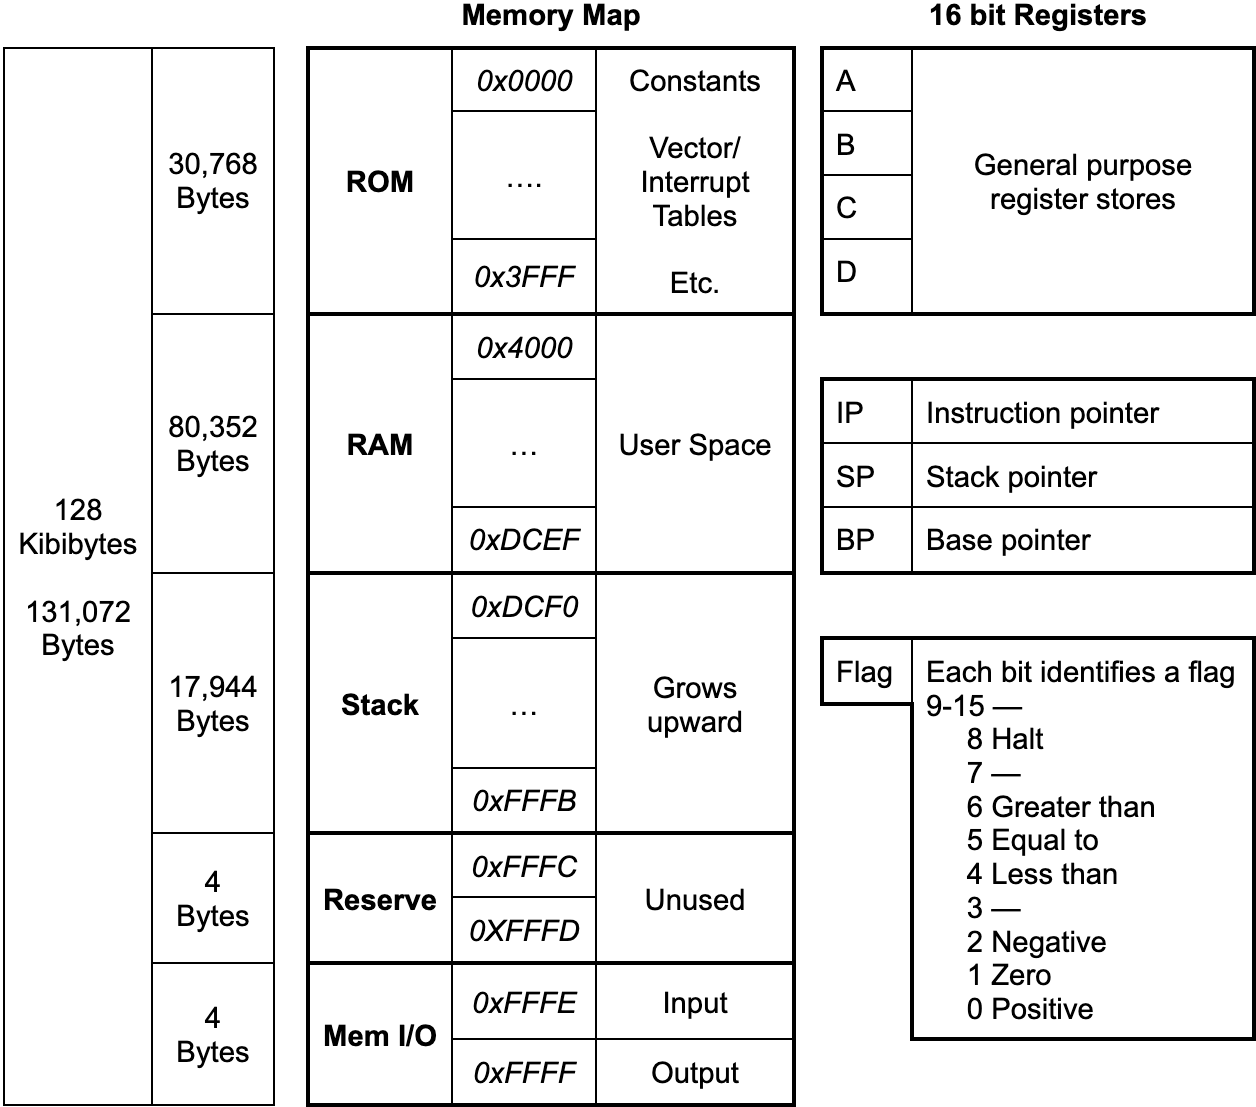
\includegraphics[width=.75\textwidth]{overview}
  \vspace*{3mm}
  \caption{A succinct overview of LLAMA-16}
  \label{fig:overview}
\end{figure}
\subsubsection{Registers}
LLAMA-16's register file contains a total of eight registers. Four are general purpose registers, three are special-use memory address registers, and one is a flags register. All registers have a 16-bit word size and all registers except the flags register are user writable. Currently, LLAMA-16's implementations are strictly virtual so retrieving data from registers or memory computationally cost the same however there are still a few reasons to use registers for operating on data opposed to solely using memory for all operations. The primary reason is the use of the flags register.\par
LLAMA-16's instruction set is intentionally overloaded allowing these instructions to operate the same regardless if the operand data is stored in a register or memory. The primary difference between operating within registers or memory is if the flags register is updated after execution. After the execution of certain instructions, namely arithmetic and logical instructions, the flags register is updated to reflect the sign of the resulting value. The flags are then used for checking conditions of data. The flags register is updated when the destination of the operation is a register; the flags register is untouched if the destination of an operation is a memory address.\par
Figure \ref{fig:flagsinstr} shows the resulting flags after each instruction in a sample program. Lines 1-2 shows the operation of subtracting $5$ from $3$ resulting in register \verb|a| holding the value of $-2$. As a result of this arithmetic operation, the \verb|negative| flag is set. Lines 3-4 shows a similar operation but the result of adding $8$ and $9$ is stored in memory at the address \verb|0x5555|. Since the result of this operation was stored in memory, the flags register was not updated. Line 5 adds the value of $17$ stored at the memory address \verb|0x5555| is added to the value $-2$ stored in register \verb|a|. Since the result of this operation, $15$, is stored in register \verb|a|, the flags register is then updated to reflect the sign of this value.\par
\begin{figure}[h]
  \centering
  \captionsetup{justification=centering}
  \begin{singlespace}
  \verb|Instruction          Resulting flags     |\\
  \rule{0.6\linewidth}{.5pt}
  \verb|1. mv #3, a           FLAGS: []           |\\
  \verb|2. sub #5, a          FLAGS: [`negative']|\\
  \verb|3. mv #8, [5555]      FLAGS: [`negative']|\\
  \verb|4. add #9, [5555]     FLAGS: [`negative']|\\
  \verb|5. add [5555], a      FLAGS: [`positive']|\\
  \end{singlespace}
  \vspace*{3mm}
  \caption{Example cases of the flags register being updated}
  \label{fig:flagsinstr}
\end{figure}
There are two reasons behind this design choice. The first is simply because there may be a case in which a programmer would want to perform an operation or a check on some data without changing the state of the conditional flags currently represented. To do this, a programmer can simply just move the data into memory and perform operations there. The second reason is to encourage programmers to write code that mimics that of modern architectures; to encourage a load/store procedure. A load/store architecture is defined as a system that loads data from memory into registers, operates on the data, and then stores the result back in memory.
\paragraph{General purpose data registers}
The four general purpose registers, identified as \verb|a|, \verb|b|, \verb|c|, and \verb|d|, are used for storing and operating on data. In a hardware implementation of traditional more complex ISAs, reading from registers is significantly faster than retrieving data from the memory bus; however this means that they are considered to be more expensive. With these more complex architectures, data is retrieved from memory, operated on within the processor's registers, and then stored back in memory. Modern processor's also have a caching scheme to temporarily save commonly retrieved data so it will be cheaper to retrieve, however this is beyond the scope of LLAMA-16's simplistic RISC design.
\paragraph{Special-use address registers}
The three special-use memory address registers are the instruction pointer (\verb|ip|), stack pointer (\verb|sp|), and base pointer (\verb|bp|) registers. The instruction pointer register holds the memory location of the next word in the current program's execution. After the current instruction is fetched from memory to be interpreted and executed, that address is incremented by one word. When execution of the current instruction has finished, the instruction stored in memory at the address stored int instruction pointer register is fetched and the cycle repeats. The stack and base pointer registers hold memory addresses of certain pointers within the machine's built-in stack. This stack is detailed further in the \hyperref[sec:stack]{The Stack} subsection. Instructions that directly modify the memory addresses in stack pointer and base pointer registers are detailed in the \hyperref[sec:stackops]{Stack Operations} paragraph of the \hyperref[sec:machineinstr]{Machine Instructions} section.
\paragraph{Flags register}
The flags register is a special-use register that is not user writable however can be read to get status information on the condition of recently modified data. Just like the other seven registers, the flags register is 16-bits wide however the data stored within these 16-bits are encoded in a special manner such that each bit represents different conditional codes. The flags can be organized into three categories: status, arithmetic, and compare flags.
\subparagraph{Status flags}
There is one status flag: the halt flag. The condition of the halt flag is checked every execution cycle. A set halt flag indicates that machine execution has been stopped. This can either be set intentionally with the halt (\verb|hlt|) instruction or can be raised by the machine itself when encountering some errors.
\subparagraph{Arithmetic flags}
The arithmetic flags are used to represent the sign of numerical data after arithmetic operations. These flags indicate whether a number is positive, negative, or zero. Since an integer has to exist in exactly one of these states, only one of these flags can be set at a time. When the flags register is checked and updated, the previous flags are first cleared before setting the correct flag.
\subparagraph{Compare flags}
The compare flags are a special subset of arithmetic flags used to represent the relationship between two integers. These flags indicate if a number is greater than, less than, or equal to another number. Just like the arithmetic flags, a relationship between two integers falls into exactly one of these categories so only one of these flags can be set at a time. These conditional flags are set by the compare (\verb|cmp|) instruction; however, in the current implementation of LLAMA-16, no other instructions can read these flags. With this in mind, the compare instruction also sets the arithmetic flags where the positive, negative, and zero flags map to the greater than, greater than, and zero flags respectively.
\subsubsection{Memory}
Memory can be thought of as a collection of storage cells with each cell storing one bit of information having the value of 0 or 1. Individually these millions of bits provide very little insight as to what the data they represent means so these bits are clustered together into more manageable chunks referred to as words. LLAMA-16's word size is 16-bits (2 bytes) meaning that all operations of the machine are conducted on 2 bytes of information at a time. LLAMA-16 also has an address bus of 16-bits meaning there are a total of $2^{16}$ (65536) addresses. Each one of these 65536 addresses can hold a 16-bit word. With $2^{16}$ addresses in the address space, each holding 2 bytes of information, the maximum possible storage capacity is 128 kibibytes. To put this in perspective, the theoretical memory limit that a 64-bit computer can address is about 18 billion gigabytes ($2^{64}$). It may seem that 128 KiB is severely limiting when compared to complex modern systems but on the other side of the spectrum of comparison, the ferrite core memory of the Gemini Digital Computer aboard the Gemini SC8 spacecraft had a storage limit of about 19.5 KiB, approximately 15\% of LLAMA-16's memory capacity \parencite{nasa}.\par
While the entire address space is readable and writable, the ISA does provide a recommended layout on how memory should be segmented. The main sections of memory are designated as general purpose `read-only-memory', general purpose random-access-memory, a recommended space for the stack, and designated memory mapped I/O addresses. See Figure \ref{fig:overview}. Read-only memory is intended to be used to store operating system functions and data structures like vector and interrupt tables. Random access memory is designated as user space for storing user programs and variables. As part of the user space, there is a recommended space allocated for the machine's stack. The last 4 bytes of memory are designated for memory mapped I/O. The stack is detailed further in \hyperref[sec:stack]{The Stack} section of this paper and more information on memory mapped I/O can be found in the \hyperref[sec:io]{Input/Output Instructions} subsection of \hyperref[sec:machineinstr]{Machine Instructions}.
\paragraph{Endianness}
Endianness refers to the order of bytes within a word. Big-endian systems store the most significant byte of a word in the smallest memory address and inversely little-endian systems store the least significant bytes in the smallest memory address. LLAMA-16 is technically a mixed middle-endian system. This means that data longer than a byte, like strings for example, are stored big-endian in sequence but within each 16-bit word, the two bytes are flipped. One way to interpret this endianness is that a string of four characters is stored as two little-endian 16-bit words with a big endian-order. See Figure \ref{fig:endianness}.
\begin{figure}[h]
  \centering
  \captionsetup{justification=centering}
  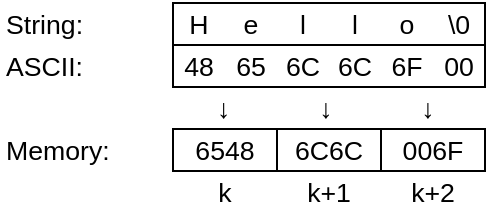
\includegraphics[width=.5\textwidth]{endianness}
  \vspace*{3mm}
  \caption{Example of string literal `Hello' stored in middle-endian}
  \label{fig:endianness}
\end{figure}
\subsubsection{Machine Instructions}
\label{sec:machineinstr}
LLAMA-16 has only sixteen unique instructions. While this may seem limiting compared to the over nine-hundred instructions available in x86\_64, sixteen is also more manageable and less daunting. There are four fields that make up an instruction: the label, mnemonic, operand(s), and the comment fields. Labels are optional for most instructions and are used to reference special instructions within the program. Labels are generally used for organizing control flow and retrieving initialized data constants. All instructions will have a mnemonic and each instruction will have a different set of valid operand types. Finally, the comment field is text used only by the human programmer. During the parsing phase of assembly, the assembler will ignore this field. LLAMA-16 mimics the AT\&T syntax style in that two operand instructions will use the first operand as a data source and the second operand is used as both a source and the destination of the resulting data. Using this style of syntax, versus the inverse Intel syntax, was an explicit design choice to make reading and writing LLAMA-16 programs more accessible. Since English speakers read and write from left to right this source-first destination-second syntax is more natural to interpret.\par
Instructions can be categorized into four groups. Data transfer instructions move data around between various locations in the machine. Data manipulation instructions modify data stored in the machine. Program sequencing instructions change the procedural control flow of program execution. Input/output instructions are used to read data from outside of the machine and output data from within the machine.
\paragraph{Data transfer instructions}
LLAMA-16's primary data transfer instruction is the move (\verb|mv|) instruction. The move instruction is intentionally designed overloaded. It is used to transfer data from and to all sources: registers, memory, and immediate data. Registers and memory locations can be used as both the source of data as well as the eventual destination of resulting data. Immediate data is data that is defined within the program, not data that can be fetched from a register or memory. Having only one instruction for nearly all data transfer drastically simplifies this category of instructions.\par
Another method of moving data is with the machine's stack. The stack is described in more detail later in this document. See subsection \hyperref[sec:stack]{The Stack}.
\paragraph{Stack operations}
\label{sec:stackops}
There are two instructions available for interacting with the stack. A program can push (\verb|push|) data onto the stack or pop (\verb|pop|) data off of the stack. When pushing 16-bit data onto the stack, the data is stored at one word past the current stack pointer. After this data is written the stack pointer is updated to point to this new data. The inverse is true when popping data off of the stack. The data is read from memory, stored wherever the instructions specifies, and then the stack pointer is decremented to the previous word. Any 16-bit word can be pushed onto the stack however when popping from the stack the data retrieved must be stored in a register or in memory as you cannot store data in an immediate value. See subsection \hyperref[sec:stack]{The Stack} for details on the data structure.
\paragraph{Data manipulation instructions}
\label{sec:dataman}
Data manipulation in the scope of the LLAMA-16 ISA entails operations that change the state of any datum stored in the machine. This includes but is not limited to bitwise logical operations and arithmetic operations. The logical operators not (\verb|not|), and (\verb|and|), and or (\verb|or|) were intentionally chosen as they are functionally complete. Functional completeness is a property of a set of logical operators where all possible truth tables can be expressed by combining members of the set into a boolean expression. While there are smaller well-known functionally complete sets of connectives, namely \verb|{AND, NOT}|, and the singleton sets \verb|{NAND}| and \verb|{NOR}|, having the `core three' connectives makes boolean algebra easier to learn and understand. For arithmetic instructions, LLAMA-16 has four. The increment (\verb|inc|) and decrement (\verb|dec|) instructions add one and subtract one respectively from the value stored at the specified operand location. These instructions are incredibly helpful when handling counter variables for loops, a common learning exercise when learning any new programming language. The other two arithmetic operators are addition (\verb|add|) and subtraction (\verb|sub|). Unlike their single operand counterparts, addition and subtraction operate on two operands. The first operand, the source, is added or subtracted to/from the second operand, the destination, and then the result is stored in the destination overwriting the original value. As an intentional design choice, the LLAMA-16 emulator does not check for overflow or underflow errors. An underflow or overflow error occurs when the result of an operation cannot be represented within the number space. For LLAMA-16 this means numbers that cannot be represented in a 16-bit signed number space. The \hyperref[sec:datarep]{Data Representation} section of this document provides more detail on underflow and overflow. This seeming flaw was intentionally left unchecked as an act to mimic modern complex computer systems. It is the job of the software to check for and handle mathematical errors. The machine can only represent data; it cannot apply meaning to it.
\paragraph{Program sequencing instructions}
There are four instructions that can be classified as program sequencing or control flow instructions. The call-subroutine (\verb|call|) and return-from-subroutine (\verb|ret|) instructions utilize the stack in a similar manner as the push and pop instructions when moving data onto/from the stack. See \hyperref[sec:stackops]{Stack Operations} subsection for details on these stack instructions. The call-subroutine instruction works by first pushing the address value currently stored in the instruction pointer register onto the stack. At the time of execution of the call-subroutine, the instruction pointer register will be storing the address of the next instruction after the call-subroutine instruction. Then, after pushing that address onto the stack, the instruction pointer register is loaded with the address of the instruction stored at the address specified by the label operand of the call-subroutine instruction and another fetch-execute cycle starts. This temporarily stores a point for execution to resume in the calling routine after completing the subroutine. To complete the routine and continue right after the jump, the return-from-subroutine instruction is used at the end of the routine. The return-from-subroutine instruction acts as the inverse to the call-subroutine instruction. It pops the address off of the stack into the instruction pointer register and execution continues on the next cycle, this time starting at the next instruction after the call-subroutine instruction.\par
The other two instructions that modify the procedural flow of a program are the jump-if-not-zero (\verb|jnz|) and halt (\verb|hlt|) instructions. The jump-if-not-zero instruction is the only conditional control instruction LLAMA-16 has. However, technically it does make the LLAMA-16 instruction set Turing-complete, aside from its bounded memory. The Church-Turing thesis is beyond the scope of this paper however a machine is considered Turing-complete if it can solve any problem that a Turing machine could solve. One of the core components of Turing-completeness is the concept that a program can control its own flow \parencite{turing}. In high level programming languages this is commonly satisfied with conditional \verb|for| and \verb|while| loops but the same effect can be achieved with \verb|GOTO| statements, recursion, and fixed-point combinators. The jump-if-not-zero instruction can be used in a similar manner as C style \verb|GOTO| statements which can be used to implement loops. LLAMA-16 can also support recursion with the call-subroutine instruction.\par
\paragraph{Input/Output instructions}
\label{sec:io}
LLAMA-16 conveniently wraps input and output functions into one instruction: \verb|io|. The second operand of the instructions specify whether data is expected to be read in (\verb|io <source>, IN|) or to write data out (\verb|io <source>, OUT|). The ISA specifies that when using this I/O instruction 16-bit words are written and read from specified memory locations. This idea of continuously reading/writing data to/from memory is referred to as memory mapped input/output. In the current implementation of the project, the only interaction available for the I/O instruction is standard input and standard output, that is, the text from the terminal running the emulator. However, the design of memory mapped I/O was chosen over other schemes like Unix file descriptors or port based I/O due to its versatility. Any device attempting to communicate with other parts of the machine can use the same memory addresses to communicate or even new addresses could be allocated for it. This also simplifies I/O operations down to just one instruction making getting user input and printing information to the user easy to implement. For comparison, in x86\_64 assembly a programmer would have to set up several registers and at least one memory location before making a system call. System calls are often considered an advanced topic in computer systems courses that rely on previous understanding of Unix files, interrupt vector tables, and signal handling. Condensing all of these concepts down to one instruction with just a few rules accelerates program writing.
\subsubsection{Instruction Representation}
\begin{figure}[h]
  \centering
  \captionsetup{justification=centering}
  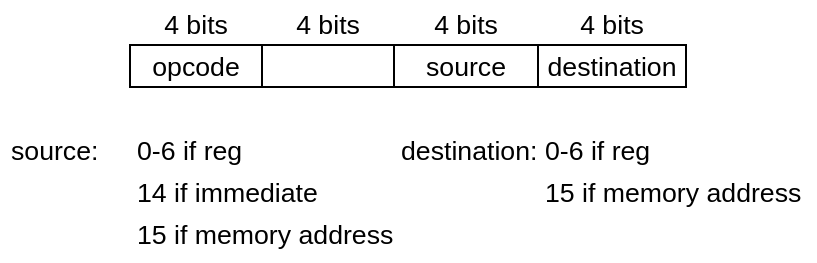
\includegraphics[width=.75\textwidth]{instrformat}
  \vspace*{3mm}
  \caption{Layout of LLAMA-16 instructions}
  \label{fig:instrformat}
\end{figure}
All of LLAMA-16's instructions are 16-bits long and are segmented into four 4-bit nybbles, each encoding specific information of the instruction. See Figure \ref{fig:instrformat}. As mentioned previously, instructions can be syntactically split into three categories: instructions with zero, one, or two operands. (Note that for the purposes of explanation the operands of two-operand instructions are referred to as the source and destination and the single operand of one-operand instructions are referred to as the source regardless if information is being moved or not). There are three types of information that can be encoded into the source and destination nybbles: whether the operand is a register, a memory address, or an immediate value. Since there are only seven registers that can be written to and read from, all registers can be represented within the 4-bit segment. The general purpose registers \verb|a|, \verb|b|, \verb|c|, \verb|d| are encoded as the decimal values 0, 1, 2, and 3 respectively. The instruction pointer, stack pointer, and base pointer registers are encoded as the decimal values 4, 5, and 6 respectively. If the operand data is stored in memory or is an immediate, this information cannot be encoded within the 4-bit segment so therefore at least one more word will be needed. The decimal value 14 is encoded to denote an immediate value and the decimal value of 15 is encoded to denote a memory address. When the emulator fetches and executes these multi-word instructions, it uses these encoding rules to determine where it will read/write the operand. Immediate data and memory addresses encodings tell the emulator to fetch the next word in the program sequence (the value stored in the instruction pointer register plus one word). In the case where both the source and destination information are stored in subsequent words, the source information will be stored in the word directly follow the instruction and the destination will be stored directly after the source.
\subsubsection{Data Representation}
\label{sec:datarep}
Since LLAMA-16's data width is 16 bits wide, one word can represent a maximum of $2^{16}$ unique objects. Depending on the context of the program running, these objects can represent a multitude of information types - text, images, colors, numbers, etc. To the machine, all data is simply a value of 16-bits; it is up to the program to determine the definition of those values. There are two main data types that can be interpreted by LLAMA-16: integers and characters.
\paragraph{Integers}
LLAMA-16 uses fixed-precision number representation meaning that all data must be represented in exactly 16 bits. As mentioned previously, 16-bit words can represent a maximum of $2^{16}$ unique objects. An issue arises when attempting to represent negative numbers in binary. Over the past 75 years, a few solutions have been developed and refined. One of those methods is Two's Complement which LLAMA-16 uses to represent signed integers. Two's complement encoding treats the most significant bit of a binary number as having a negative weight. In the case of 16-bit numbers, the most significant bit has a weight of $-2^{16}$. Arithmetically, this truncates the maximum number that can be represented to $2^{16-1}$ however, it allows for the range of possible numbers to be extended into the negative number space: a range from $-2^{12-1}$ to $2^{16-1}-1$ (-32768 to 32767).
\paragraph{Characters}
To a computer all information is simply a string of bits meaning that non-numerical data, like characters, must be encoded as numbers so the machine can interpret them. One of the earliest standards developed to do this is called ASCII: American Standard Code for Information Interchange. ASCII is a specified rule set for encoding and decoding characters for machine readability. ASCII was originally developed for teletypes in 1963 so some of the original functionality is no longer commonplace but it still acts as the de-facto basis for all character representation.
\subsubsection{The Stack}
\label{sec:stack}
A stack is an abstract data type used as a collection of elements in a sequence. A stack is a last in, first out collection meaning that the data that was last pushed onto the stack is the only data that is accessible. To the machine, the stack is simply data in memory. The difference between this data and any other data in memory is that there are specific pointers to sections of the stack. The stack pointer register holds the memory address of the data currently on the top of the stack. The base pointer register holds a memory address of something significant to the program or programmer. At initialization the stack pointer and base pointer registers hold the same address as without storing any data no space needs to be allocated. When pushing data onto the stack; the value in the stack pointer register is incremented by one word. When popping data from the stack, the value in the stack pointer register is decremented by one word. The base pointer serves a slightly different function. At initialization the base pointer points to the bottom of the stack however this can be manually updated by user programs to create a structure within the stack. One common application of this allocating space for function variables. When changing the base and stack pointers to point to a location slightly beyond the current data in the stack it creates a bubble of space for subroutines and user programs to store temporary data.\par
The stack is also used when executing subroutines. When the call-subroutine instruction is executed, the address of the next program instruction is pushed onto the stack and the address of the instruction referenced by the label operand is moved into the instruction pointer register. This indicates that the next cycle of execution will start somewhere else in the program. When that subroutine is finished the return-from-subroutine instruction will pop the return address from the stack in the instruction pointer register and execution will continue where it left off in the calling procedure.
\subsection{Assembler Design}
An assembler acts as the bridge between symbolic instructions coded by a programmer and the machine code read by the processor. Assemblers read one line of the source program at a time and attempt to translate those symbolic instructions to machine code. Both the assembler and the emulator are written in standard library Python with a minimum version of 3.6. The assembler heavily utilizes Python's dynamic string methods to parse, search, and substitute strings read from the source file. A parser for a more complex assembler or compiler would generally implement a Look-Ahead-Left-to-Right or a recursive descent parsers however, the computational theory of efficient parsing is beyond the scope of this project. Instead, the LLAMA-16 assembler treats each line of the source program as independent from all other lines. Once a line has been parsed successfully, its tokens are saved, and the next line is parsed.Since all assembly statements follow the same structure, the assembler only needs to tokenize up to five tokens per line.\par
\vspace{5mm}
\begin{figure}[h]
  \centering
  \captionsetup{justification=centering}
  \verb|[label:] [mnemonic [operand1[, operand2]]] [;comment]|
  \vspace*{3mm}
  \caption{Structure of a line of LLAMA-16 assembly}
\end{figure}
The LLAMA-16 assembler parses each line right to left. This may seem counter-intuitive, but since labels are an optional field and mnemonics are not, parsing right to left ensures that the assembler correctly tokenizes the mnemonic and label separate instead of incorrectly parsing the mnemonic as the label. The assembler starts by removing any white space from the beginning and ending of the line and then checks to see a semicolon (;) exists anywhere in the line. A semicolon is used to denote a comment, so if a semicolon exists the assembler knows that everything to the right is comment and can be safely disregarded. Next, the string left of the semicolon is checked for comma. A comma is used to separate the two operands of an instruction. The string that is to the right of that comma is the second operand. If there is no comma to be found, then the second operand is set to an empty string. The first operand is parsed by checking for any white space character (i.e. a tab or a space). Finally, to split the label field from the mnemonic field, the assembler looks for a colon (:) character. If no colon character is found, then the line does not have a label and the field is set to an empty string. LLAMA-16's assembler is classified as a two-pass assembler meaning the source program is parsed and tokenized twice.
\paragraph{Pass one}
On the first pass, the assembler reads one line at a time and generates machine code for the instruction. For most instructions, this process works just fine. The assembler has a dictionary of all instructions, registers, memory addresses, and knows how to interpret immediate data. When it comes across symbolic tokens of these types, it will translate them directly to machine code. However, if the assembler comes across a label that it has not seen before, it does not have a definition so translation is not possible yet. To work around this, an auxiliary data structure called a symbol table is used.
\paragraph{Symbol table}
The symbol table is a data structure utilized by the assembler to keep track of variable labels found in the source file. Labels are used to reference specified instructions within the program are helpful for organizing control flow and retrieving initialized data constants. Since labels can be any string that the programmer chooses and can reference any section of code anywhere in the program, the assembler does not have a predefined definition for these constants. The first time the assembler sees a label, it will record it and the address it can be found at in the table. This allows further translation to occur without knowing the definition of the label.
\paragraph{Pass two}
Once the assembler has finished the first scan of the source program, it will scan the source again starting from the beginning. At this point, most of the program has been translated; however the placeholder values of the labels need to be updated. On the second pass, the assembler rescans the source looking for untranslated labels. When it encounters one, it will reference the newly generated symbol table for its definition and finish translation.
\paragraph{Learning options}
The assembler features a few debugging options to help illustrate its functionality. The first is the option to display each line's tokens (the label, mnemonic, operands, and comment) as well as the line number of operand types. This can be used to understand how the assembler is reading the programs. Another feature is the ability to save the symbol table to a human readable file. This is also helpful when attempting to understand how the assembler is interpreting the programs. The symbol table is also shown after parsing each line. With this, users can see step by step the process the assembler is taking to translate the source programs.
\subsection{Emulator Design}
LLAMA-16's emulator is designed to be a machine emulator meaning it's structured in such a way that it is program independent. Any program successfully assembled for LLAMA-16 can be run on the emulator. The emulator features a number of debugging tools to give users the opportunity to learn what program execution looks like in real time. To run a LLAMA-16 program with the emulator, users pass the assembled binary as a command line argument. An instance of the emulator is created specifically for that program; the emulator closes after execution is finished. The \hyperref[sec:os]{Operating system} subparagraph of the \hyperref[sec:futurework]{Future Work} section details an alternative feature to make emulation more seamless.
\paragraph{Memory}
At a high-level, memory is simply a long array of cells where data can be stored and retrieved. In the case of this emulator, memory is literally a long array of cells. The array is of length $2^{16}$, each representing an addressable memory location. Each location stores an unsigned 16-bit integer representing the encoded binary data stored at each location. Reading and writing to memory is encapsulated in an Object-Oriented manner where a Memory object is created and modified with class methods. This simplifies the processor methods that execute the machine instructions. The emulator also features the ability to get a memory map after program execution. To do this, all non-zero values are formatted to the more human readable notation of hexadecimal and are printed to standard out.
\paragraph{Processor}
The main component of any computer is the processor. The LLAMA-16 emulator is designed to mimic how hardware would interpret the machine code. The register file, holding the values of all registers on the machine, is represented using an array of unsigned 16-bit integers. Registers can be written to and read from in a similar manner to memory. The instruction pointer register, stack pointer register, and base pointer registers are special-use registers however they look identical to any other register. Safeguarding these registers was intentionally omitted from the design as to accurately emulate a machine. The same philosophy is applied to safeguarding against overflow and underflow errors. See subsection \hyperref[sec:dataman]{Data manipulation} instructions for details on over/underflow error checking.
\paragraph{Learning options}
LLAMA-16's emulator also features a number of options to help users gain a better understanding of the execution cycle. Since LLAMA-16's emulator is currently only a command line based interface, an option is available for printing processor state information after every execution cycle. The emulator also features an option to view the memory map of the machine during and after program execution.
\section{Testing and Validation}
Two sets of tests were used to check for errors in the assembler and emulator. The first set of tests were to check the correct output of the assembler. Eighteen assembly files were created: one per instruction and another two for the \verb|.string| and \verb|.data| directives. Within an assembly file, each line consisted of one combination of operands valid for that file's instruction. For example, the \verb|add.asm| test file contained six lines of instructions each with a valid combination of immediate values, registers, and memory addresses for the addition instruction. See Figure \ref{fig:addtest}.  The binary output of these assembly files were first hand compiled using the specifications of the ISA. Utilizing the Linux \verb|hexdump| utility, the binary data from the assembler was compared against the hand compiled expected output.\par
\vspace*{3mm}
\begin{figure}[h]
  \centering
  \captionsetup{justification=centering}
  \begin{singlespace}
  \verb| add #2, a          ; immediate, register|\\
  \verb|add #2, [5555]     ; immediate, memory  |\\
  \verb|add a, b           ; register, register |\\
  \verb|add a, [5555]      ; register, memory   |\\
  \verb|add [5555], a      ; memory, register   |\\
  \verb|add [5555], [6666] ; memory, memory     |\\
  \end{singlespace}
  \vspace*{3mm}
  \caption{Testing program of the addition instruction used to test the assembler}
  \label{fig:addtest}
\end{figure}
The next set of testing assembly files were a collection of simple programs using various LLAMA-16 instructions in conjunction. These programs are meant to test the assembler and emulator end-to-end. Each one was designed to mimic actual use cases of the instruction set. Each program only used a small subset of instructions so that errors could be easily traced. First, each program was hand compiled using the ISA specifications. These programs were checked for assembler accuracy by comparing the binary data to the expected binary data, just like the previous set. Next, each program was assembled and emulated with multiple sets of different parameters. The output of these programs was captured and compared against the expected output. Examples such programs were subtraction resulting in negative integers, addition resulting in overflow errors, calling of multiple subroutines, and pushing and popping different data types onto and off of the stack.
\section{User Verification and Feedback}
A lab activity working with LLAMA-16 was given to computer science students in UNC Asheville's Systems II class on November 1, 2022. The activity handout detailed a brief overview of the LLAMA-16 ISA, a small collection of example programs, and access to the repository's documentation. A short presentation was given demonstrating the usage of the assembler and the emulator. Students were tasked with writing an iterative Fibonacci calculator for LLAMA-16. The specification of the assignment was to prompt the user for an integer, iteratively calculate its corresponding Fibonacci number, and print the result out to the user. Of the ten students in the class working on the assignment, nine were able to develop a working solution within a class period and all ten submitted working solutions before the due date the following day. While detecting edge cases and protecting against underflow/overflow errors was not part of the assignment, a number of student submissions did handle at least one of the major edge cases: detecting zero input, detecting negative input, detecting non-integer input, or managing overflow errors.\par
Some qualitative feedback was also given by students. One comment given by a student was in regards to the operand syntax of LLAMA-16: ``The only thing I found confusing is that the source and destination are backwards from what we have been using [in previous Systems II labs] (S. Hendricks, personal communication, November 3, 2022).'' The concern of using the AT\&T style vs the Intel style of syntax was the subject of a question from another student during the lab: ``Why use the AT\&T style when the Intel style is more prevalent? (M. Kothe, personal communication, November 1, 2022).'' The reasoning behind the choice of AT\&T vs Intel was readability by new assembly programmers. Since English speakers read left to right, the logical flow of moving data from the left-most operand to the right-most operand is easier to understand. However, in the case of a few students in this Systems II class who had had a little exposure to x86 assembly, a brief clarification was needed when first attempting to write LLAMA-16 programs. This could be a point of contention for an educational tool however there is no definitive answer in the debate between Intel and AT\&T syntax.\par
One student said that they enjoyed the exploratory nature of the project, mentioning that it was a nice low-pressure introduction to assembly programming: ``I found working through the lab to be an engaging experience as I could see the immediate effect of the machine instructions I used for the program\ldots. Being able to view the effect of the machine instructions and interact with them through the code made the function and format of each of the instructions we used easier to memorize and replicate, as opposed to just reading them from the book or looking them up online (J. Alpizar, personal communication, November 20, 2022).''
\section{Future Work}
\label{sec:futurework}
While LLAMA-16's small feature set is rich in versatility, the project is far from completion. A number of useful features could be added to the project to further refine its ability to act as an educational tool.
\paragraph{Macro assembler}
A macro assembler is an assembler that generates code from predefined macros. A macro assembler would allow users to write programs with a larger instruction set without changing the underlying architecture. Macro defined instructions would also be an enhancement of the instruction set and would not be required to be learned to utilize the project's tools.
\paragraph{Visualization}
In the current implementations of the emulator users only have access to a text based interpretation of the machine through representations of the machine's state. A GUI application with various panels visually displaying the cycle of instruction fetching, instruction decoding, execution, memory access, and register write back in real time would help to further explain the process of machine code execution.
\paragraph{Operating system}
\label{sec:os}
One of the in development features is a simple lightweight operating system. This OS would allow users to load and run programs from within the emulator rather than passing a program to the emulator as a command line argument from the host system. Users could ``boot-up'' the emulator like a real computer and interact with programs and data through a command line interface. This would offer a more streamline exploration process for users since they would be able to interact with the ``machine'' directly. Such command line utilities could include the ability to poke values directly into memory, peeking at specific memory addresses, viewing and setting environment variables like clock speed and the ability to look at the processes of instruction level parallelism. The operating system could be written in the LLAMA-16 instruction set or could be abstracted in a higher level language as part of the emulator itself.
\printbibliography
\end{document}
